\subsection{Electrical components}

Any electrical hardware consists of a number of components that are connected to each other. In this case, the most important type of component is the boolean logic gate \texttt{NAND}. In addition to that, several of the logical modules and components have been abstracted away by the software simulation system. In these systems, tasks such as clock generation and memory access control are implicit. In the electrical implementation, these must be explicitly built from a set of components. Likewise, an electrical implementation must consider functionalities of purely electrical significance such as power management and circuit protection. Also, while the idea behind the project is to build the internal logic entirely from individual \texttt{NAND} logic gates, this is unnecessary for components that are not visually interesting or do not provide significant educational value. This chapter provides a brief overview of all used electrical components and their purpose. 

Since all useful electrical circuits use passive components such as capacitors, resistors and inductors of multiple values and sizes, these will not be explored in detail here. All of the passive components use a 0402 package, as it is the smallest and cheapest package available for automated assembly in most consumer-grade assembly houses.

\begin{wrapfigure}{r}{0.4\textwidth}
    \centering
    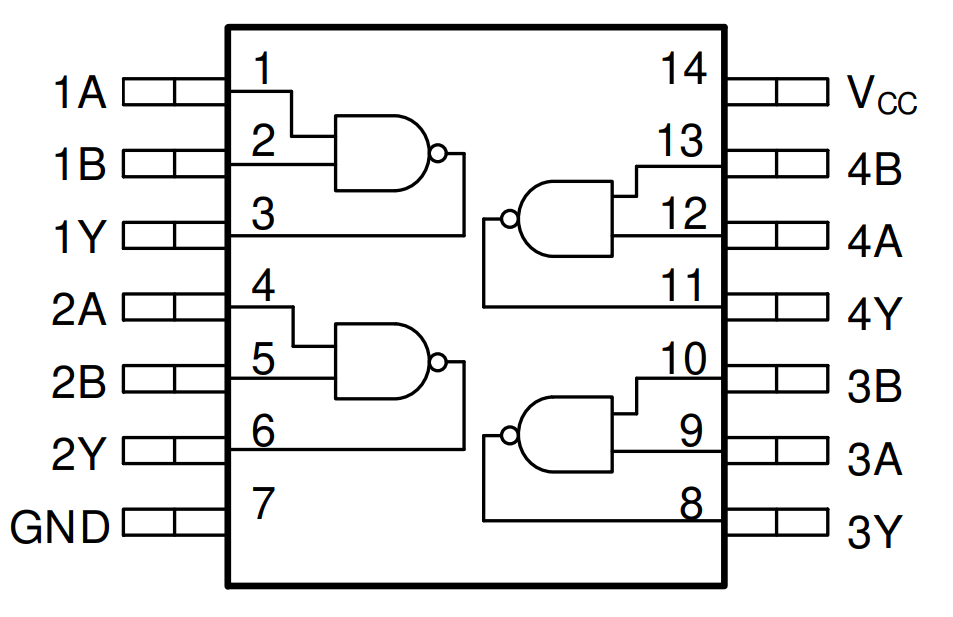
\includegraphics[width=0.38\textwidth]{images/SN74HC00_pinout.png}
    \caption{Functional pinout and internal gate layout of the SN74HC00 IC (SNx4HC00 datasheet, Rev. H \cite[p. 1]{ti_sn74hc00})}
    \label{fig:hardware_components_sn74hc00_pinout}
\end{wrapfigure}\leavevmode

\subsubsection{NAND gate}

The primary component of the device is the individual \texttt{NAND} logic gate. However, while \acp{ic} of this type are available, each individual gate \ac{ic} requires a power supply and ground pin in addition to the signal pins. For this reason, the majority of such 2 input logic gate \acp{ic} contain four gates per chip. this way, these four gates can share their supply and ground pins, decreasing complexity and number of connections required. For this reason, the ``SN74HC00'' \ac{ic} by Texas Instruments is chosen. \autoref{fig:hardware_components_sn74hc00_pinout} shows the layout of the four contained gates, as well as the pin mapping for their inputs and outputs. The chip is part of the ``SN74'' family of chips, multiple of which are used in this work. By using components from the same family, it is more likely for different components to work together well. This family of components has been available since 1982, providing the additional advantage of being readily available, well known and well documented. 

\subsubsection{Multiplexer}

Multiplexers are an example of a component with a repetitive internal structure. For this reason, they will not be built from individual logic gates. Instead, ``SN74HC157'' \acp{ic} are used. Each chip provides a 4 bit 2:1 multiplexer in a single \ac{ic}. This chip is used in every multiplexer used to interconnect a logical module, as is explained in \autoref{fig:implementation_interconnection_datapath}. It also replaces the multiplexers used for bit shifting and result selection within the \ac{alu}. In total, two 16 bit 2:1 multiplexers and eleven 8 bit 2:1 multiplexers are replaced. This is equivalent to one 120 bit 2:1 multiplexer. This requires 120 individual 1 bit 2:1 multiplexers. Since each \ac{ic} provides four such multiplexers, a total of $120 / 4 = 30$ \acp{ic} is needed. As each a 2:1 multiplexer requires four \texttt{NAND} gates, and each SN74HC00 contains exactly four gates, this would require a total of $120 * 4 / 4 = 120$ chips. Therefore, using a premade multiplexer \ac{ic} reduces the number of components used four-fold.

\subsubsection{Memory}

All memory components use parallel data and address interfaces. Even though the \ac{rom} used to store control signals is only indexed by the seven bits of each opcode, it uses the same chip as the program \ac{rom}, which uses the full 16 bit address space. This is done in order to use as few distinct components as possible. Even so, the pinout and packages of many \acp{rom} are intercompatible in accordance to \ac{jedec} 21-C \cite[not publicly available]{jedec_jesd21c}. In this standard, the pin mapping for memories using the DIP-32 package is defined so that memories of different address space sizes can use the same access circuitry. The standard defines 19 pins to be used for addressing. If a memory provides less than that, the most significant bits can simply be left unconnected internally. An external device accessing the memory will then see the contents of the available region ``mirrored'' in higher regions. A practical example is the memory layout of the original GameBoy console. The memory region \texttt{C000 - DFFF} is mirrored at \texttt{E000 - FFFF} \cite[chapter 1.4, page 15]{nintendo_gb_manual_v1_1} due to this mechanism. Programmers developing software for the device call this region ``Shadow RAM'', since its use is not recommended by the manufacturer.

The configuration and layout of data pins is also standardised. All data pins are bidirectional in a bus-style interface, as explained in \autoref{sec:fundamentals_busses}. Like the address and data signals, the set of control signals is also standardised. This even extends to the type of memory. For this reason, it is possible to interchange \ac{ram} and non-volatile \ac{rom} chips. This allows contents of ``RAM'' to be inspected even when the device is no longer powered. Since all memories are using the same pin layout and are relatively expensive, they are used in combination with sockets. This way, memories can be replaced and reused. Also, programs and instruction sets can be switched out by replacing the relevant \acp{rom}.

For the volatile memories in this work, the ``AS6C4008-55PCN'' by Alliance Memory is chosen. It provides a low access time of \SI{55}{\nano\second} for both reads and writes\cite[page 1]{alliance_as6c4008}. For the non-volatile memories, the ``SST39SF040'' by Microchip Technologies is chosen. It has the same low read access time of \SI{55}{\nano\second}. However, writing to the device is far slower. Typical rewrites of the whole address space take up to \SI{8}{\second}\cite[page 1]{microchip_sst39sf040}. However, this increases only the time needed for installing programs or instruction sets, for which \SI{8}{\second} is deemed fast enough. Both types of memoriy follow the \ac{jedec} standard for DIP-32 memories and are interchangeable while using the full 19 bit address space. If not available, variants with lower capacity can be substituted at the cost of lower maximum program size and working \ac{ram}, respectively.

\subsubsection{Connectors}

A hardware implementation is likely split up into modules, similar to the way the logical device is. Therefore, these modules must be connected in order to share data, power and control signals. For this work, simple \SI{2.54}{\milli\meter} pitch headers and sockets are used. These are widely available, cheap, hand-solderable and mechanically stable. They provide the additional advantage of being trimmable to the required length. This way, only one length of connector needs to be purchased, reducing overall cost and number of distinct components. Connectors of this type are rated to carry \SI{3}{\volt} of continuous \ac{dc}\cite{multicomp_2213r_series}, which is more than enough for this project, even for power supply pins. If more current is required, multiple such pins can be used in parallel to carry a shared load. They are also available in vertical grid-layouts, providing a higher signal density per unit of board edge.

In order to deliver power to the device, a standard \SI{5.5}{\milli\meter} \ac{dc} barrel jack is used. It can handle continuous currents of up to \SI{5}{\ampere} at \SI{12}{\volt}\cite{cliff_dc_connectors}. In addition to the barrel jack, a \ac{usb} type B connector is used for providing a programming interface for the user. A \ac{usb} 3.0 connector can also carry up to \SI{900}{\milli\ampere} at \SI{5}{\volt}. However, having a separate power supply allows a much wider range of power supplies and voltages to be used. The \ac{usb} signal is internally converted to \ac{uart} using an ``FT32RL'' \ac{ic} by FTDI. Both the \ac{usb} and barrel jack connectors provide circuit protection by integrating mechanical reverse polarity protection.

\subsubsection{Mechanical input}

To interface with the user, mechanical inputs are needed. To enable user input, simple tactile switches are used. They are cheap and readily available. However, like all mechanical switches, they suffer from signal bouncing. In such mechanical switches, some physical contacts have to approach each other at finite speeds. Therefore, the imperfect surfaces of the contacts create arcing and do not touch instantaneously. This results in an oscillation of the output signal until it settles into the new state. \autoref{fig:hardware_components_switch_bounce} shows a simplified example of bouncing within a switch circuit due to these phenomena.

\begin{figure}[h!]
    \centering
    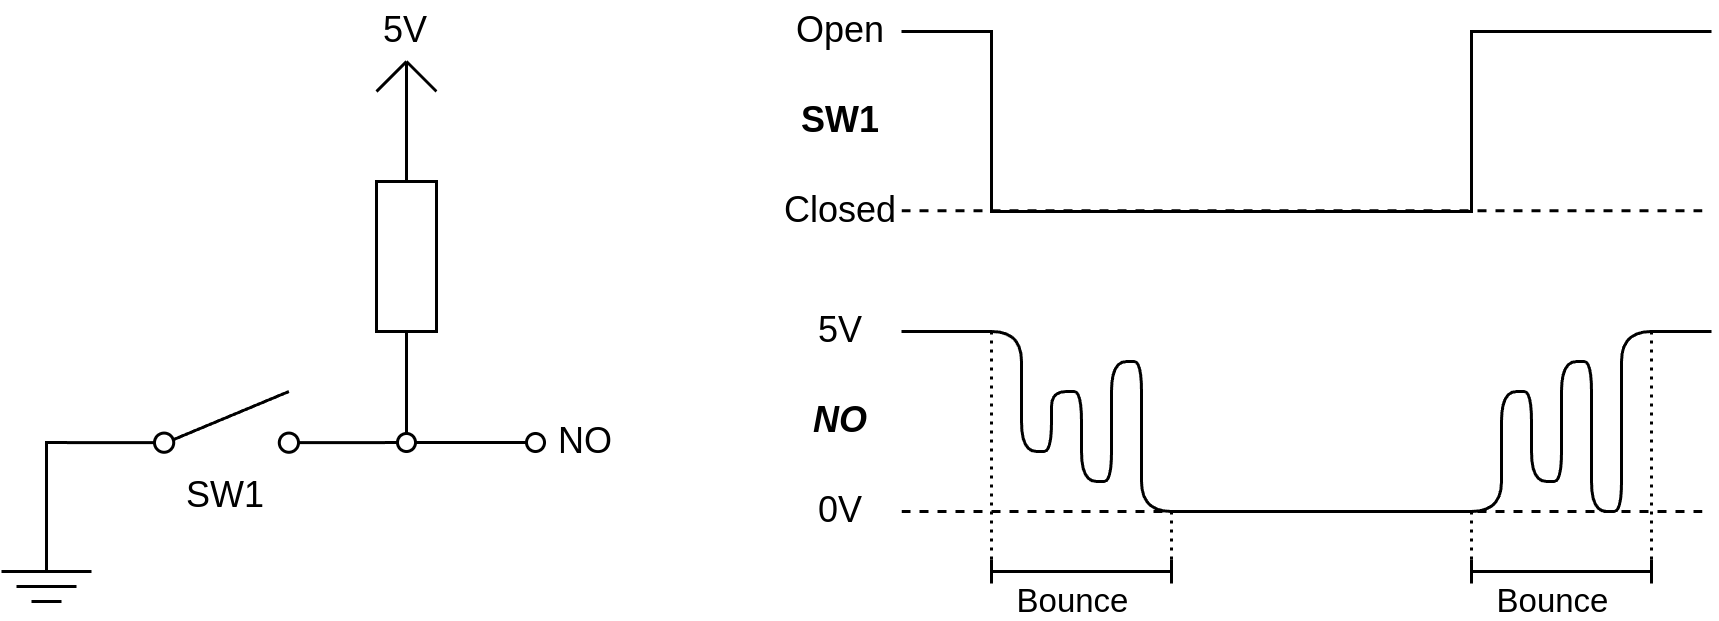
\includegraphics[width=0.8\textwidth]{images/drawio/switch_bounce.png}  % Replace with your image file
    \caption{Bouncing switch circuit and the graphs for mechanical position and output signal (Modified from Clive Maxfield of Digikey Electronics, omitted description of bounces and outline of switch \cite{maxfield_hardware_debounce})}
    \label{fig:hardware_components_switch_bounce}
\end{figure}

The bouncing output is unsuitable for further processing. Therefore, a debouncing circuit is introduced. It uses an RC-member to smooth the output signal, as well as a Schmitt Trigger to output a signal with clean, near-instant edge transitions. This circuit is shown in \autoref{fig:hardware_components_switch_debounce}. The output signal of the switch is smoothly transitioned into its new state over time due to the capacitor charging or discharging. Once the capacitor charge has reached a certain level, the Schmitt Trigger toggles its output signal to the new state, too. As seen in the last graph, the output corresponds to the idealised input signal, only shifted by the time it takes the capacitor to charge. For this project, the ``SN74HC14'' by Texas Instruments is used for this purpose, since it provides six Schmitt Triggers within one package and is also part of the same family of logic \acp{ic} as the logic gates and multiplexers.

\begin{figure}[h!]
    \centering
    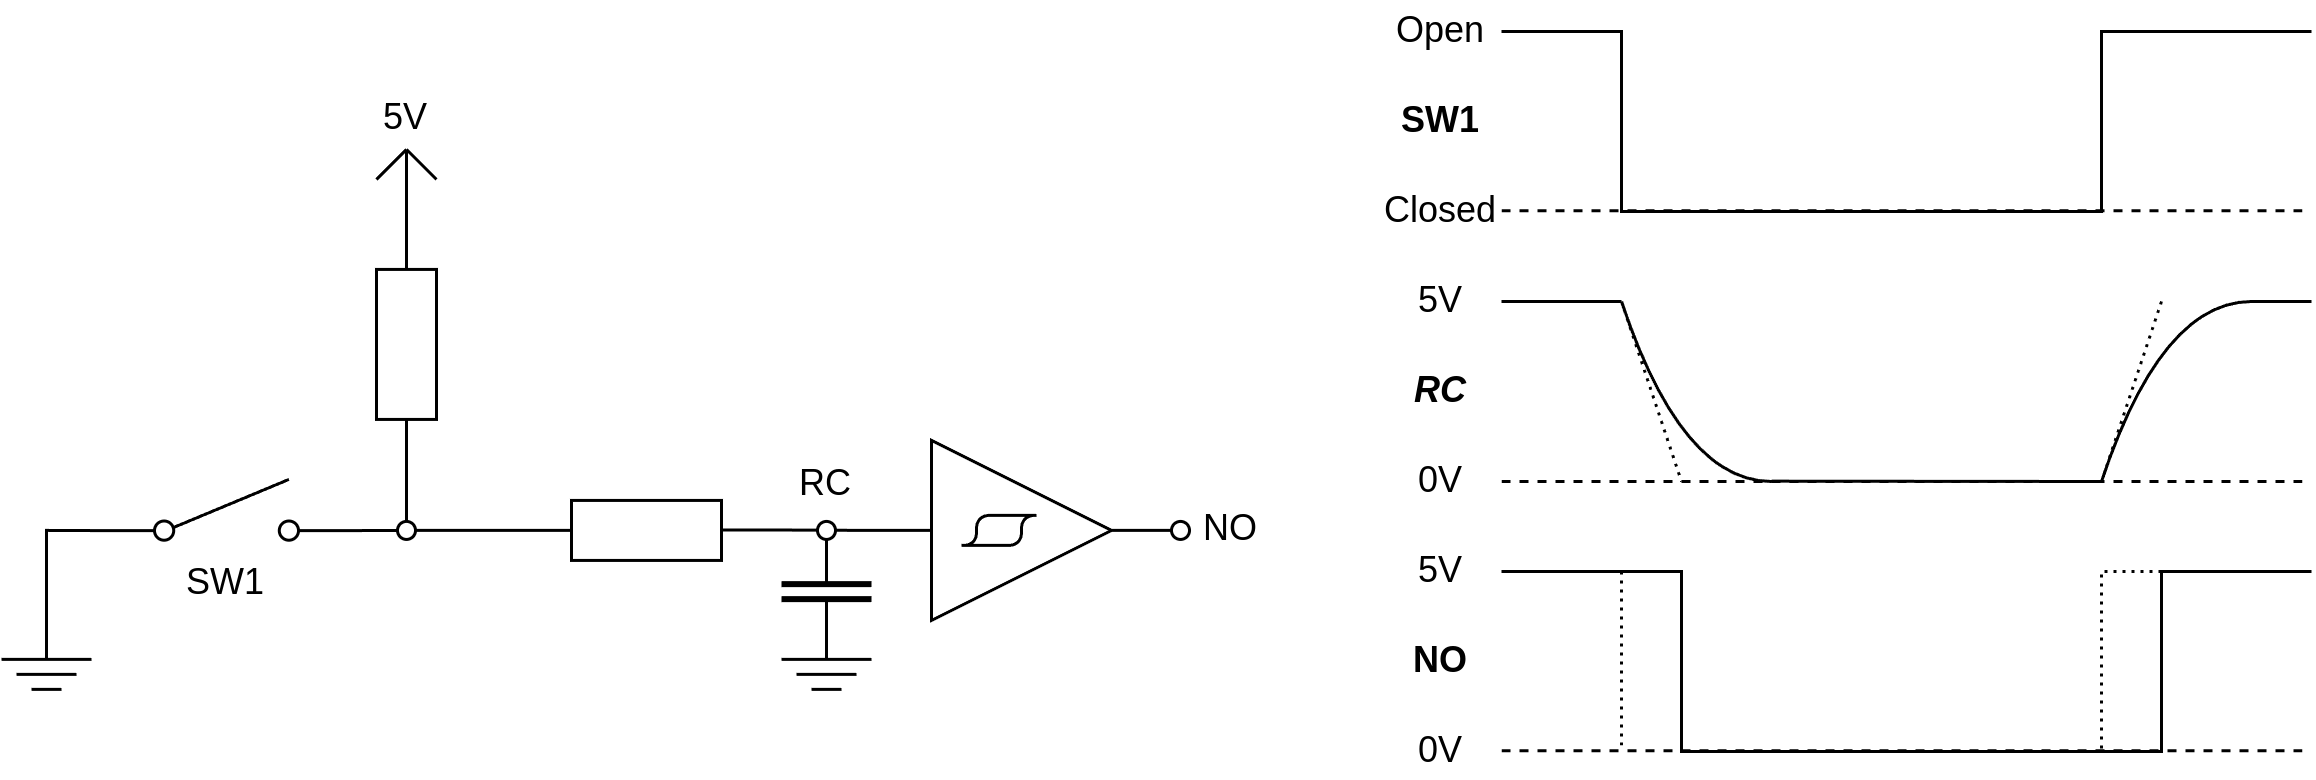
\includegraphics[width=0.9\textwidth]{images/drawio/switch_debounce.png}  % Replace with your image file
    \caption{Switch debouncing circuit using an RC member and Schmitt Trigger}
    \label{fig:hardware_components_switch_debounce}
\end{figure}

\subsubsection{LED}

In addition to user input, the state of the device should be displayed using a visual interface. For this purpose, \acp{led} are used. They are cheap, readily available, silent and require low power to produce a significantly visible output. If needed, they can be driven at a visible frequency or using a \ac{pwm} signal in order to differentiate between multiple states per \ac{led}. Again, these are standard components that are available in many packages, colors and forward voltage and current configurations. For this project, 0402-\acp{led} with a forward voltage of \SI{3}{\volt} are used and driven at a current of \SI{2}{\milli\ampere}. This requires one \SI{1}{\kilo\ohm} resistor per \ac{led}.

\subsubsection{Circuit protection}

The external power connector must be protected against electrotechnical faults such as reversed polarity or overvoltages. For this reason, additional components are introduced. A ``TSR 3N'' switching regulator by Traco Power converts an input voltage of \SI{4.6}{\volt} - \SI{36}{\volt} to a stable output voltage of \SI{5}{\volt} \cite{tracopower_tsr3}. Its output is the primary power source for the entire device. A standard \SI{5}{\milli\meter} $\times$ \SI{20}{\milli\meter} fuse is used directly behind the positive output of the \ac{dc} barrel jack. An alternative is a \ac{ptc} device such as a polyfuse. However, since the total current draw of the device can only estimated, a soldered device such as a polyfuse is harder to replace than a regular fuse. For inverting, amplifying or decoupling binary input and output signals, \acp{mosfet} are used. Both N and P channel variants are needed to cover different use cases. The ``IRLML6402'' and ``IRLML6244'' by Infineon are chosen, respectively, due to past positive experiences.

\subsubsection{Arbiter}

In the software simulation, the clock signal is generated implicitly. However, in the electrical implementation, some component must generate the clock signal for all \ac{cpu} modules. For this purpose, an integrated \ac{mcu} is used. This \ac{mcu} is referred to as the ``arbiter'', as it represents the system at the highest level of control within the entire \ac{cpu}. For this work, the ``ATMega2560'' by Microchip Technologies is used, as it offers 86 \ac{gpio} pins, is widely available, well documented and runs at \SI{5}{\volt}. It is also compatible with the ``Arduino'' framework, which provides libraries for all functions of the chip, reducing software development time. The usage and role of the arbiter is explained in more detail in \autoref{sec:hardware_arbiter}.

